\documentclass[twocolumn]{article}
\usepackage{graphicx}
\usepackage{amsmath}
\usepackage{amsthm}
 
\theoremstyle{definition}
\newtheorem{definition}{Definition}[section]

% Recap the problem and motivation. This part should be brief, since we've already
% heard about this.

% Briefly describe your overall approach. A small concrete example snippet or two
% would be very helpful.

% Results. Describe what you have achieved. What remains to be done to make this a
% full-fledged research result?

% Lessons Learned. Reflect on the work you did, so you and I can learn from it.
% How did your approach differ from what you originally proposed, and why? What
% was more (or less) challenging than you expected? What would you do differently
% next time? What do you now see as the strengths/weaknesses of a tool like Coq,
% and what does that imply about possible research directions to pursue?

% Code. Please submit all of your Coq code along with some brief documentation so
% I can relatively easily play with it and understand what's going on.
\title{Verified Sentential Decision Diagrams}
\author{Steven Holtzen\\Saketh Ram Kasibatla}
\date{\today}
\begin{document}
\maketitle

\section{Introduction and Motivation}
The goal of this project is to construct and reason about sentential decision
diagrams (SDDs) in Coq. A sentential decision diagram is a data structure which encodes
an arbitrary Boolean formula; see Fig.\ref{fig:sdd} for an example SDD. 

\begin{figure}
  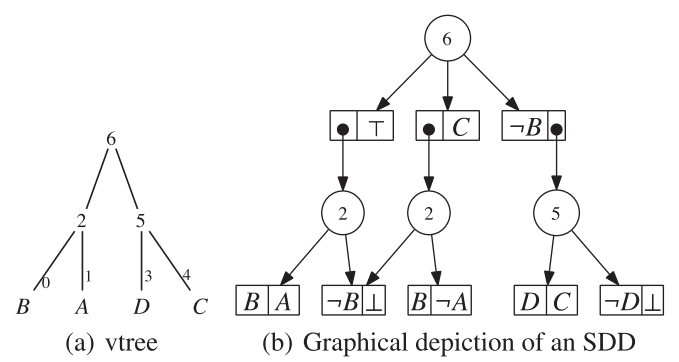
\includegraphics[width=\linewidth]{sdd.png}
  \caption{An SDD for the Boolean formula $f = (A \land B) \lor (B \land C) \lor
    (C \land D)$. Reproduced from \cite{Darwiche2011}.}
  \label{fig:sdd}
\end{figure}

The SDD data structure has several desirable properties:
\begin{enumerate}
\item Canonicity. Any two equivalent Boolean formulas will always compile to
  the same SDD.
\item Determinism. Any given Or-node in an SDD will have at most one true
  child.
\item Decomposability. The children of any given And-node in an SDD share
  no variables.
\end{enumerate} 
These properties allow one to perform many queries in linear time the SDD data
structure, for example: model enumeration, weighted model counting,
satisfiability and validity checking. In our work, we focused on non-canonical
(i.e. uncompressed) SDDs, which are easier to represent and manipulate.

The key operations that we focused on implementing were (1) SDD compilation; 
(2) SDD application; (3) SDD evaluation. 

\subsection{Proof Goals}
Our original goal was to prove the following properties:
  \begin{enumerate}
  \item Correctness: For all Boolean formalae $e$ and inputs $i$,
    \texttt{eval\_boolexpr}($e$, $i$) =
    \texttt{eval\_sdd}(\texttt{compile}($e$),  $i$).
  \item Prove that the resulting SDD is decomposable.
  \item Prove that the resulting SDD is deterministic.
  \item Prove that \texttt{init\_var} generates SDDs with respect to the same
    $v$-tree (will most likely be a necessary lemma for proving the correctness
    of \texttt{apply}).
  \end{enumerate} 
During the course of implementation, these goals proved to be too ambitious. We
were able to prove, subject to certain assumptions, that SDDs remain
decomposable after application; See Fig. \ref{fig:decomposable}. We relaxed goal (1) to be to prove a particular
property of the SDD post-application; see Fig.\ref{fig:unsatthm}.

\begin{figure}
\begin{verbatim}
Theorem sdd_decomposable :
  forall sdd v,
    sdd_vtree sdd v ->
    vtree_correct v ->
    decomposable sdd.
\end{verbatim}
  \caption{Theorem around decomposability}
  \label{fig:decomposable}
\end{figure}

\begin{figure}
\begin{verbatim}
Theorem apply_unsat :
  forall sdd1 sdd2 sddres,
    sdd_unsat sdd1 ->
    sdd_apply OAnd sdd1 sdd2 sddres ->
    sdd_unsat sddres.
\end{verbatim}
  \caption{The apply unsat theorem.}
  \label{fig:unsatthm}
\end{figure}
The proof of this fact required a custom inductive hypothesis on the derivation
of \texttt{sdd\_apply}, which we will elaborate on in later sections. The reason
that this approach can not be extended to prove stronger claims and possbile
future work will also be discussed.

\section{Approach}

\subsection{OCaml Prototype and Fixpoints vs. Inductive Constructions}
We created an initial OCaml implementation of SDD compilation and application to
guide our Coq implementation. This implementation can be found in the
\texttt{ml/} directory of the project.

Some key observations of this OCaml code is that it is reasonably complex; a
direct translation of this code to Gallina was attempted, but ultimately we
decided against it for the following reasons.

\begin{itemize}
\item It was difficult to establish that all the recursive calls (especially
  \texttt{apply}) provably terminated.
\item It is difficult to reason about Gallina code, as we would have had to prove many assumptions from the code, before being able to reason about its correctness.
\end{itemize} 

Instead, we opted to specify the SDD data structure as an inductive in Gallina, and to specify operations on this data structure using inductive relations. This approach allowed us immediate access to assumptions that were integral to proving the theorems we were interested in, and made it easy to strengthen these assumptions as necessary.

\subsection{Inductive SDD Data Structure}
We used the following compact definition for our SDD datastructure:

\begin{verbatim}
Inductive atom : Type :=
| AFalse : atom
| ATrue : atom
| AVar :  nat -> bool -> atom.

Inductive sdd : Type :=
| Or: list (sdd * sdd) -> sdd
| Atom : atom -> sdd.
\end{verbatim}
An \texttt{or} node is simply a list of pairs $(p_i, s_i)$ (primes and subs).

\subsection{SDD V-Tree}\label{sec:vtree}
We experimented with (1) representing the V-Tree as a dependent type of the SDD
and (2) creating a seperate \texttt{sdd\_vtree : sdd -> vtree} inductive relation which
generates a V-Tree from a particular SDD:

\begin{verbatim}
Inductive sdd_vtree : sdd -> vtree -> Prop :=
| AtomTrue : forall n, 
 sdd_vtree (Atom ATrue) (VAtom n)
| AtomFalse : forall n, 
 sdd_vtree (Atom AFalse) (VAtom n)
| AtomVar : forall n b, 
 sdd_vtree (Atom (AVar n b)) (VAtom n)
| OrEmpty : forall v, sdd_vtree (Or []) v
| OrSingle: forall prime sub lvtree rvtree tail, 
 sdd_vtree prime lvtree ->
 sdd_vtree sub rvtree ->
 sdd_vtree (Or (tail)) (VNode lvtree rvtree) ->
 sdd_vtree (Or ((prime, sub) :: tail)) 
  (VNode lvtree rvtree)

\end{verbatim}

This relation is used throughout our proofs as a correctness assumption. A valid SDD must obey some V-Tree.

\subsection{SDD Application}
SDD application is the process of combining two SDDs $\alpha$ and $\beta$ into a
third SDD $\gamma$ according to some operation $\circ$. We defined application
as a 4-argument inductive relation:
\begin{verbatim}
Inductive sdd_apply : 
  op -> sdd -> sdd -> sdd -> Prop
\end{verbatim}

where \texttt{op} is either $\land$ or $\lor$. We decomposed this relation in 3
mutually recursive sub-relations:
\begin{enumerate}
\item \texttt{atom\_apply}, which handles applying together atoms
\item \texttt{apply\_or\_list}, which takes two SDD \textt{or}-nodes as arguments and
  produces a new SDD \texttt{or}-node.
\item \texttt{apply\_single\_list}, which takes a prime $p$, a sub $s$, and an
  \texttt{or}-node $[(p_i, s_i)]$ as an argument and produces the SDD of the
  form $[(p_i \land p, s_i \circ s)]$ for all $i$, where $\circ$ is applying
  \texttt{op}.

  For this operation, if $p_i \land p$ is not satisfiable, it is not to be
  included in the final \texttt{or}-node which is produced. This necessitates
  an \texttt{sdd\_sat} and \texttt{sdd\_unsat} relations.
\end{enumerate}

\subsection{Custom Inductive Hypothesis}
Ultimately in order to prove theorems of the form in Fig\ref{fig:unsatthm}, we
need to be able to decompose along the primes and subs of the SDD. Because we implemented \texttt{or}-nodes' children as lists of pairs of nodes, the default inductive hypothesis that Coq inferred for the SDD datastructure, and for the \texttt{sdd\_apply} inductive construction proved too weak. These default inductive hypotheses failed to break down the lists of primes and subs embedded in our SDD data structure.

To resolve this issue, we created custom inductive hypotheses for the SDD data structure, and for the \texttt{sdd\_apply} inductive construction (\texttt{sdd\_ind'} and \texttt{sdd\_apply\_ind'} respectively). Refer to the attached source code for implementations of these hypotheses. Each of these hypotheses contains a fixpoint which operates on the proof goal. When the user calls the tactic \texttt{induction sdd using sdd\_ind'}, she is asked to prove the goal, in relation to each prime and sub. The machinery of the custom inductive hypothesis then builds a proof of the general goal, using proofs of each piece. In such a manner, \texttt{sdd\_apply\_ind'} gave us inductive hypotheses strong enough to prove \texttt{apply\_unsat}.

\subsection{SDD Compilation}
SDD compilation is the process of transforming a Boolean expression into an SDD.
This procedure requires the following components:
\begin{enumerate}
\item An implementation of Boolean expressions. (\texttt{BoolExpr.v})
\item A method which generates an sdd from an atom (\texttt{sdd\_of\_atom})
\end{enumerate}

We compile SDDs from boolean expressions in a bottom-up fashion. First, each atom is turned into an SDD atom. Then, we use \texttt{sdd\_apply} to combine these atoms according to the boolean expression (and them together for each and node, or them together for each or node).

\subsection{Decomposability}

Our proof of decomposability relies heavily on varSets (implemented in \texttt{VarSet.v}). For any SDD or vtree, we can obtain a varSet, which is the set of all variables mentioned in the SDD/vtree. We prove decomposability by showing that the varSet of an SDD is a subset of the varSet of any vtree it obeys (see \texttt{sdd\_vtree\_vars}). We then use this result, along with induction on the \texttt{sdd\_vtree} relation to prove the theorem shown in Fig. \ref{fig:decomposable}. Interestingly, we did not need a custom inductive hypothesis to prove this property, as the \texttt{sdd\_vtree} relation encoded enough information about how to decompose the SDD and vtree in question to push the proof through.

\section{Results}

Our final codebase contains the following inductive constructions:

\begin{itemize}
\item \texttt{sdd\_apply}
\item \texttt{sdd\_vtree}
\item \texttt{sdd\_sat}
\item \texttt{sdd\_unsat}
\item \texttt{sdd\_of\_var}
\item \texttt{sdd\_eval}
\item Judgements around varSets (see \texttt{VarSet.v} and judgements containing \texttt{\_varSet} in \texttt{IndSdd.v})
\item Judgements around boolean expressions (see \texttt{BoolExp.v})
\end{itemize}

We successfully proved \texttt{sdd\_unsat} and \texttt{sdd\_decomposable}, using custom inductive hypotheses and inductive relations on sdds and vtrees. 

In order to make our codebase a full research result, we would need to prove:

\begin{itemize}
\item apply preserves vtree - that the operands and result of the \texttt{sdd\_apply} operation all obey the same vtree. This result, combined with our proof of decomposability would be enough to show that any compiled SDD is decomposable
\item determinism (as formulated in the original goals)
\item correctness (also as formulated in the original goals).
\end{itemize}

Together, these properties would prove that our implementation of SDDs is valid, and would be enough to make our implementation a point of comparsion for other researchers.

\section{Lessons Learned}

\subsection{Challenges}

* use inductive judgements from the start
* include useful data as arguments (pass vtree to apply)
* seek the simplest implementation for proofs

\subsection{Strengths and Weaknesses of Coq}

* need a strong grasp of theory and complex type systems
  - dependent types
  - curry howard isomorphism
* bad UX
  - want to look at multiple points in a proof
  - want to organize hypothesis
  - want to see data structures and proof judgements


\bibliographystyle{plain}
\bibliography{bib}
\end{document}
